% WT-HALI: Write-Through Hierarchical Adaptive Learned Index
% ELL405 Operating Systems Course Project - FINAL VERSION

\documentclass[aspectratio=169,10pt]{beamer}
\usetheme{Madrid}

% Packages
\usepackage{tikz}
\usepackage{pgfplots}
\usepackage{booktabs}
\usepackage{amsmath}
\usepackage{graphicx}
\usepackage{colortbl}
\usepackage{array}
\usepackage{hyperref}

\usetikzlibrary{shapes,arrows,positioning,fit,calc}
\pgfplotsset{compat=1.17}

% Clickable links
\hypersetup{
    colorlinks=true,
    linkcolor=blue,
    urlcolor=blue
}

% Title Information
\title[WT-HALI]{WT-HALI: Write-Through Hierarchical Adaptive Learned Index}
\subtitle{Benchmarking Traditional and Learned Index Structures}
\author[Dhruv Joshi, Anushka Chaturvedi]{
    Dhruv Joshi (2022EE32079)\\
    Anushka Chaturvedi (2022EE31763)
}
\institute[IIT Delhi]{
    ELL405: Operating Systems\\
    Indian Institute of Technology, Delhi
}
\date{Fall 2025}

% Remove footer
\setbeamertemplate{footline}{}
\setbeamertemplate{navigation symbols}{}

\begin{document}

% ============================================================
% TITLE SLIDE
% ============================================================
\begin{frame}
\titlepage
\end{frame}

% NO OUTLINE SLIDE - removed as requested

% ============================================================
% SECTION 1: INTRODUCTION
% ============================================================

\begin{frame}{Motivation: The Index Problem}
\textbf{Indexes are critical for database and file system performance}

\vspace{0.3cm}

\begin{columns}
\column{0.5\textwidth}
\textbf{Traditional Indexes}
\begin{itemize}
    \footnotesize
    \item B+Tree, Hash Table, ART
    \item Fast, well-understood
    \item Higher memory (19-42 B/key)
    \item 3-5 cache misses typical
    \item \textcolor{green!70!black}{13-17M inserts/sec}
\end{itemize}

\column{0.5\textwidth}
\textbf{Learned Indexes}
\begin{itemize}
    \footnotesize
    \item ML models predict positions
    \item \textcolor{green!70!black}{Low memory (16 B/key)}
    \item 70-200ns lookups
    \item \textcolor{red}{Only 180K ins/sec}
    \item Requires periodic retraining
\end{itemize}
\end{columns}

\vspace{0.4cm}

\begin{center}
\colorbox{blue!10}{\parbox{12cm}{\centering
\textbf{Goal:} Achieve learned index memory efficiency without sacrificing write throughput.\\[0.1cm]
\footnotesize \textbf{Our contribution:} WT-HALI achieves \textcolor{green!70!black}{5$\times$ faster writes} than pure learned indexes while maintaining 16.7 B/key memory efficiency.
}}
\end{center}
\end{frame}

\begin{frame}{Project Overview}
\textbf{Benchmark suite: 6 index structures across 108 experiments}

\vspace{0.2cm}

\begin{columns}
\column{0.55\textwidth}
\begin{columns}
\column{0.48\textwidth}
\begin{block}{Traditional}
\scriptsize
\begin{itemize}
    \item B+Tree
    \item Hash Table
    \item ART (Radix Tree)
\end{itemize}
\end{block}

\column{0.48\textwidth}
\begin{block}{Learned}
\scriptsize
\begin{itemize}
    \item PGM-Index
    \item RMI
\end{itemize}
\end{block}
\end{columns}

\vspace{0.1cm}

\begin{block}{Our Contribution: WT-HALI}
\scriptsize
\begin{itemize}
    \item Hybrid: Binary search router + Adaptive experts
    \item Write-through ART buffer for fast inserts
    \item 100\% routing accuracy (vs 25-47\% in v1)
\end{itemize}
\end{block}

\column{0.42\textwidth}
\textbf{Write Performance Comparison:}
\begin{center}
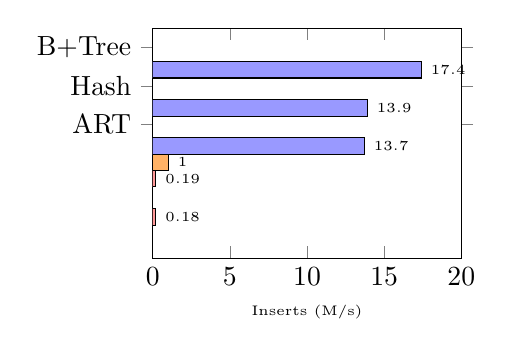
\begin{tikzpicture}
\begin{axis}[
    xbar,
    width=5.5cm, height=4.5cm,
    xlabel={\tiny Inserts (M/s)},
    symbolic y coords={PGM, RMI, WT-HALI, ART, Hash, B+Tree},
    ytick=data,
    xmin=0, xmax=20,
    bar width=6pt,
    nodes near coords,
    every node near coord/.append style={font=\tiny},
    ytick style={font=\tiny},
    xlabel style={font=\tiny}
]
\addplot[fill=blue!40] coordinates {(17.4,B+Tree) (13.9,Hash) (13.7,ART)};
\addplot[fill=orange!60] coordinates {(1.0,WT-HALI)};
\addplot[fill=red!40] coordinates {(0.19,RMI) (0.18,PGM)};
\end{axis}
\end{tikzpicture}
\end{center}
{\tiny WT-HALI: 5$\times$ better than learned indexes}
\end{columns}
\end{frame}

% ============================================================
% SECTION 2: OS CONTEXT AND BACKGROUND
% ============================================================

\begin{frame}{Indexes in Operating Systems}
\textbf{Why indexing matters for OS design}

\vspace{0.15cm}

\begin{columns}
\column{0.48\textwidth}
\begin{block}{File Systems}
\scriptsize
\begin{itemize}
    \item \textbf{XFS:} B+Trees for inodes, extents, free space
    \item \textbf{Btrfs:} Copy-on-Write B+Trees throughout
    \item \textbf{NTFS:} B+Trees for MFT and directory indexing
    \item \textbf{ext4:} HTree (hash-based) for large directories
    \item \textbf{ZFS:} Hash tables + B+Trees for metadata
\end{itemize}
\textit{Requirements:} Crash recovery, concurrency, range queries
\end{block}

\begin{block}{Database Systems}
\scriptsize
\begin{itemize}
    \item PostgreSQL, MySQL/InnoDB, SQLite: B+Tree indexes
    \item Query optimizer depends on predictable index costs
    \item ACID transactions require consistent index behavior
\end{itemize}
\end{block}

\column{0.48\textwidth}
\begin{block}{OS Design Principles at Stake}
\scriptsize
\begin{enumerate}
    \item \textbf{Simplicity:} Kernel code must be auditable\\
          {\tiny B+Tree: $\sim$1000 LOC vs WT-HALI: 2000+ LOC}
    \item \textbf{Worst-case guarantees:} O(log N) always\\
          {\tiny Not ``usually fast'' — tail latency matters for SLAs}
    \item \textbf{Predictability:} Same input $\rightarrow$ similar latency\\
          {\tiny B+Tree: 1.4$\times$ variance vs WT-HALI: 8$\times$}
    \item \textbf{Proven reliability:} 50+ years of B+Tree\\
          {\tiny Battle-tested in every major OS and DBMS}
\end{enumerate}
\end{block}

\vspace{0.1cm}

\begin{center}
\colorbox{yellow!20}{\scriptsize \textbf{Core tension:} Memory efficiency vs Performance predictability}
\end{center}
\end{columns}

\vspace{0.1cm}

\begin{center}
\colorbox{blue!10}{\scriptsize \textbf{Research question:} Can learned indexes offer meaningful trade-offs for OS/DB indexing?}
\end{center}
\end{frame}

\begin{frame}{Why B+Trees Dominate: The Baseline}
\textbf{Understanding what we're competing against: 22ns lookups, 17M ins/sec}

\vspace{0.2cm}

\begin{columns}
\column{0.6\textwidth}

\textbf{Cache-Friendly Design:}
\begin{itemize}
    \scriptsize
    \item Node size = 64 bytes (exactly one cache line)
    \item Fanout 16-32 $\rightarrow$ only 3-4 tree levels for millions of keys
    \item Sequential leaf pointers enable efficient range scans
    \item CPU prefetching works well with predictable traversal
\end{itemize}

\vspace{0.15cm}

\textbf{Write-Optimized Operations:}
\begin{itemize}
    \scriptsize
    \item Node splits are \textbf{local} — no global restructuring required
    \item No model retraining — structure adapts incrementally
    \item Fine-grained locking enables high concurrency
    \item Easy WAL/journal integration for crash recovery
\end{itemize}

\vspace{0.15cm}

\textbf{Predictable Performance:}
\begin{itemize}
    \scriptsize
    \item \textbf{Guaranteed} O(log N) worst-case for all operations
    \item Data-distribution independent: works on any workload
    \item Latency variance only 1.4$\times$ across distributions
\end{itemize}

\column{0.38\textwidth}
\begin{center}
\textbf{Latency Comparison:}

\vspace{0.2cm}

\scriptsize
\begin{tabular}{lrr}
\toprule
\textbf{Index} & \textbf{Min} & \textbf{Max} \\
\midrule
B+Tree & 20ns & 28ns \\
WT-HALI & 79ns & 636ns \\
\bottomrule
\end{tabular}

\vspace{0.3cm}

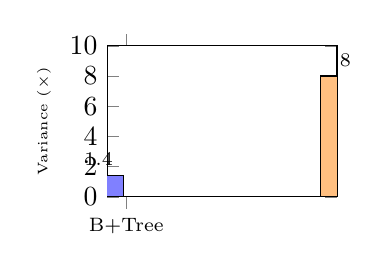
\begin{tikzpicture}
\begin{axis}[
    ybar,
    width=4.5cm, height=3.5cm,
    ylabel={\tiny Variance ($\times$)},
    symbolic x coords={B+Tree, WT-HALI},
    xtick=data,
    xticklabel style={font=\scriptsize},
    ymin=0, ymax=10,
    bar width=18pt,
    nodes near coords,
    every node near coord/.append style={font=\scriptsize},
    ylabel style={font=\tiny}
]
\addplot[fill=blue!50] coordinates {(B+Tree,1.4)};
\addplot[fill=orange!50] coordinates {(WT-HALI,8.0)};
\end{axis}
\end{tikzpicture}

{\tiny Lower variance = predictable tail latency}
\end{center}
\end{columns}

\vspace{0.1cm}

\begin{center}
\colorbox{yellow!20}{\scriptsize \textbf{Hypothesis:} Can we trade some predictability for memory savings in constrained environments?}
\end{center}
\end{frame}

\begin{frame}{What are Learned Indexes?}
\begin{center}
\textit{``An index is a model that maps keys to positions''} — Kraska et al., SIGMOD 2018
\end{center}

\vspace{0.2cm}

\begin{columns}
\column{0.42\textwidth}
\textbf{Traditional B+Tree:}
\begin{enumerate}
    \scriptsize
    \item Start at root, navigate via child pointers
    \item Compare keys at each internal node
    \item Binary search within leaf node
\end{enumerate}
{\scriptsize \textit{Cost:} 3-5 cache misses, 19-42 B/key}

\vspace{0.25cm}

\textbf{Learned Index:}
\begin{enumerate}
    \scriptsize
    \item Train model $f$ on (key, position) pairs
    \item At query: compute $pos = f(key)$
    \item Binary search in error range $[pos \pm \epsilon]$
\end{enumerate}
{\scriptsize \textit{Cost:} 2-4 cache misses, 16 B/key}

\vspace{0.2cm}

\colorbox{red!15}{\parbox{5cm}{\centering \scriptsize
\textbf{The Write Problem:}\\
Inserts require array shifts + model retraining\\
B+Tree: 17M/s vs Learned: 180K/s\\
\textbf{$\sim$100$\times$ slower!}
}}

\column{0.55\textwidth}
\begin{center}
\textbf{Linear Model Approximation:}

\vspace{0.15cm}

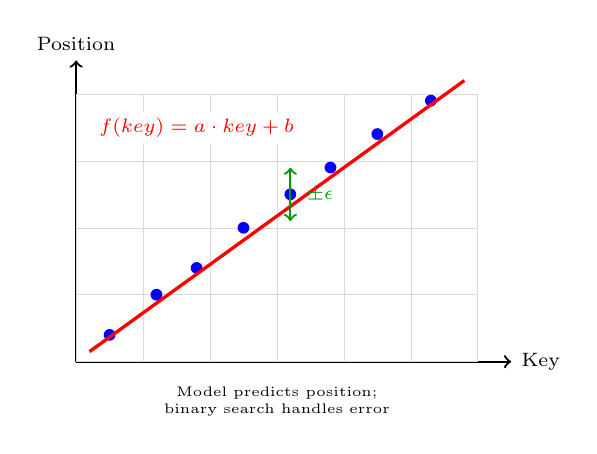
\begin{tikzpicture}[scale=0.85]
% Axes
\draw[->, thick] (0,0) -- (6.5,0) node[right] {\scriptsize Key};
\draw[->, thick] (0,0) -- (0,4.5) node[above] {\scriptsize Position};

% Grid
\draw[gray!30, very thin] (0,0) grid (6,4);

% Data points
\foreach \x/\y in {0.5/0.4, 1.2/1.0, 1.8/1.4, 2.5/2.0, 3.2/2.5, 3.8/2.9, 4.5/3.4, 5.3/3.9} {
    \fill[blue] (\x,\y) circle (2.5pt);
}

% Linear fit
\draw[red, very thick] (0.2,0.15) -- (5.8,4.2);

% Error range illustration
\draw[<->, green!60!black, thick] (3.2,2.1) -- (3.2,2.9);
\node[green!60!black, right, font=\scriptsize] at (3.3,2.5) {$\pm\epsilon$};

% Label - positioned to avoid intersection
\node[red, fill=white, inner sep=2pt, font=\scriptsize] at (1.8,3.5) {$f(key) = a \cdot key + b$};

% Annotation
\node[font=\tiny, text width=3cm, align=center] at (3,-0.6) {Model predicts position;\\binary search handles error};
\end{tikzpicture}
\end{center}
\end{columns}
\end{frame}

% ============================================================
% SECTION 3: HALI DESIGN - THE JOURNEY
% ============================================================

\begin{frame}{HALI v1: Our First Attempt}
\textbf{Initial idea: Combine RMI routing with adaptive experts and a delta buffer}

\vspace{0.2cm}

\begin{columns}
\column{0.55\textwidth}
\begin{center}
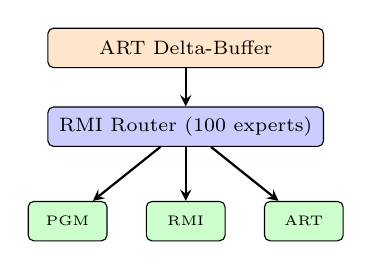
\begin{tikzpicture}[
    box/.style={draw, rectangle, minimum height=0.5cm, font=\scriptsize, rounded corners=2pt},
    arrow/.style={->, thick, >=stealth}
]
% Delta buffer
\node[box, fill=orange!20, minimum width=3.5cm] (buffer) at (0,2.5) {ART Delta-Buffer};

% RMI Router
\node[box, fill=blue!20, minimum width=3.5cm] (router) at (0,1.5) {RMI Router (100 experts)};

% Experts
\node[box, fill=green!20, minimum width=1cm] (pgm) at (-1.5,0.3) {\tiny PGM};
\node[box, fill=green!20, minimum width=1cm] (rmi) at (0,0.3) {\tiny RMI};
\node[box, fill=green!20, minimum width=1cm] (art) at (1.5,0.3) {\tiny ART};

% Arrows
\draw[arrow] (buffer) -- (router);
\draw[arrow] (router) -- (pgm);
\draw[arrow] (router) -- (rmi);
\draw[arrow] (router) -- (art);
\end{tikzpicture}
\end{center}

\vspace{0.1cm}

\textbf{The Design:}
\begin{itemize}
    \scriptsize
    \item RMI model routes queries to one of 100 experts
    \item Each expert is PGM, RMI, or ART based on data fit
    \item Delta buffer absorbs new inserts
    \item Periodic merge + retrain
\end{itemize}

\column{0.42\textwidth}
\begin{block}{Results (Clustered, 500K keys)}
\scriptsize
\begin{center}
\begin{tabular}{lrr}
\toprule
\textbf{Metric} & \textbf{HALI v1} & \textbf{B+Tree} \\
\midrule
Lookup & 507 ns & 23 ns \\
Insert & 1.2 M/s & 17 M/s \\
Memory & 16 B/key & 19.2 B/key \\
Routing acc. & \textcolor{red}{25-47\%} & N/A \\
\bottomrule
\end{tabular}
\end{center}
\end{block}

\vspace{0.1cm}

\begin{alertblock}{Why It Failed}
\scriptsize
\begin{enumerate}
    \item \textcolor{red}{Router accuracy only 25-47\%}
    \item Misprediction $\rightarrow$ must scan multiple experts
    \item Overlapping key ranges caused ambiguity
    \item RMI router itself needed retraining
\end{enumerate}
\end{alertblock}
\end{columns}

\vspace{0.1cm}

\begin{center}
\colorbox{red!15}{\scriptsize \textbf{Lesson:} Probabilistic routing is unacceptable for indexing — we need deterministic guarantees}
\end{center}
\end{frame}

\begin{frame}{HALI v1 $\rightarrow$ v2: The Critical Fix}
\textbf{Key insight: Replace probabilistic RMI router with deterministic binary search}

\vspace{0.15cm}

\begin{columns}
\column{0.48\textwidth}
\begin{block}{v1 Problem: Probabilistic Routing}
\scriptsize
\begin{itemize}
    \item RMI \textit{predicts} which expert handles a key
    \item Prediction accuracy: only 25-47\%
    \item On misprediction: must check neighbors
    \item Key ranges \textbf{overlap} between experts
\end{itemize}
\end{block}

\begin{block}{v2 Solution: Deterministic Routing}
\scriptsize
\begin{itemize}
    \item \textbf{Disjoint} key ranges: Expert $i$ owns $[b_i, b_{i+1})$
    \item Binary search on boundaries: O(log $m$)
    \item \textcolor{green!70!black}{100\% routing accuracy guaranteed}
    \item Write-through buffer for all inserts
\end{itemize}
\end{block}

\column{0.48\textwidth}
\begin{center}
\textbf{Performance Comparison:}

\vspace{0.15cm}

\scriptsize
\begin{tabular}{lrr}
\toprule
\textbf{Metric} & \textbf{v1} & \textbf{v2} \\
\midrule
Lookup & 507 ns & 636 ns \\
Insert & 1.2 M/s & \textcolor{green!70!black}{\textbf{10.2 M/s}} \\
Routing acc. & 25-47\% & \textcolor{green!70!black}{\textbf{100\%}} \\
\bottomrule
\end{tabular}

\vspace{0.2cm}

\textbf{The Trade-off:}

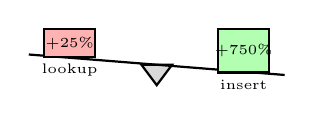
\begin{tikzpicture}[scale=0.65]
% See-saw visualization
\draw[thick, fill=gray!30] (3,0) -- (3.3,0.4) -- (2.7,0.4) -- cycle;
\draw[thick] (0.5,0.6) -- (5.5,0.2);

% Left side (slower lookups)
\draw[thick, fill=red!30] (0.8,0.55) rectangle (1.8,1.1);
\node[font=\tiny] at (1.3,0.82) {+25\%};
\node[font=\tiny] at (1.3,0.3) {lookup};

% Right side (faster inserts)  
\draw[thick, fill=green!30] (4.2,0.25) rectangle (5.2,1.1);
\node[font=\tiny] at (4.7,0.67) {+750\%};
\node[font=\tiny] at (4.7,0) {insert};
\end{tikzpicture}
\end{center}
\end{columns}

\vspace{0.1cm}

\begin{center}
\colorbox{green!15}{\parbox{12cm}{\centering \scriptsize
\textbf{Key insight:} We sacrifice 25\% lookup latency to gain 8.5$\times$ write throughput\\
\textit{Note: 10.2M/s is buffer-only; end-to-end with merges averages 1.0M/s}
}}
\end{center}
\end{frame}

\begin{frame}{WT-HALI: Final Architecture}
\begin{center}
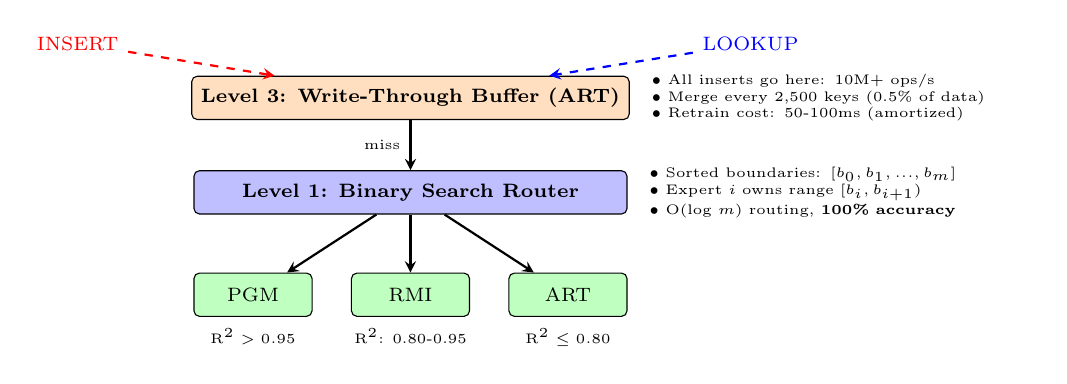
\begin{tikzpicture}[
    box/.style={draw, rectangle, minimum height=0.55cm, font=\scriptsize, rounded corners=2pt},
    arrow/.style={->, thick, >=stealth}
]

% Level 3: Buffer
\node[box, fill=orange!25, minimum width=5.5cm] (buffer) at (0,3) {
    \textbf{Level 3: Write-Through Buffer (ART)}
};
\node[right=0.15cm of buffer, font=\tiny, text width=4.8cm, align=left] {
    $\bullet$ All inserts go here: 10M+ ops/s\\
    $\bullet$ Merge every 2,500 keys (0.5\% of data)\\
    $\bullet$ Retrain cost: 50-100ms (amortized)
};

% Level 1: Router
\node[box, fill=blue!25, minimum width=5.5cm] (router) at (0,1.8) {
    \textbf{Level 1: Binary Search Router}
};
\node[right=0.15cm of router, font=\tiny, text width=4.8cm, align=left] {
    $\bullet$ Sorted boundaries: $[b_0, b_1, ..., b_m]$\\
    $\bullet$ Expert $i$ owns range $[b_i, b_{i+1})$\\
    $\bullet$ O(log $m$) routing, \textbf{100\% accuracy}
};

% Level 2: Experts
\node[box, fill=green!25, minimum width=1.5cm] (pgm) at (-2,0.5) {PGM};
\node[box, fill=green!25, minimum width=1.5cm] (rmi) at (0,0.5) {RMI};
\node[box, fill=green!25, minimum width=1.5cm] (art) at (2,0.5) {ART};

\node[below=0.03cm of pgm, font=\tiny] {R$^2 > 0.95$};
\node[below=0.03cm of rmi, font=\tiny] {R$^2$: 0.80-0.95};
\node[below=0.03cm of art, font=\tiny] {R$^2 \leq 0.80$};

% Arrows
\draw[arrow] (buffer) -- node[left, font=\tiny] {miss} (router);
\draw[arrow] (router) -- (pgm);
\draw[arrow] (router) -- (rmi);
\draw[arrow] (router) -- (art);

% Input labels
\node[above left=0.2cm and 0.8cm of buffer, font=\scriptsize, red] (ins) {INSERT};
\node[above right=0.2cm and 0.8cm of buffer, font=\scriptsize, blue] (look) {LOOKUP};
\draw[arrow, red, dashed] (ins) -- (buffer);
\draw[arrow, blue, dashed] (look) -- (buffer);

\end{tikzpicture}
\end{center}

\vspace{0.1cm}

\begin{columns}
\column{0.48\textwidth}
\textbf{Lookup Path:}
\begin{enumerate}
    \tiny
    \item Check ART buffer first (100-200ns)
    \item If miss: binary search router finds expert
    \item Expert predicts position $\rightarrow$ local binary search
\end{enumerate}

\textbf{Insert Path:}
\begin{enumerate}
    \tiny
    \item Insert directly into ART buffer — O(log $n$)
    \item When buffer $>$ 2,500 keys: merge + retrain experts
\end{enumerate}

\column{0.48\textwidth}
\textbf{Adaptive Expert Selection:}
\begin{itemize}
    \tiny
    \item R$^2$ coefficient measures linear fit quality
    \item High R$^2$ ($>$0.95): use PGM (fast, memory-efficient)
    \item Medium R$^2$ (0.80-0.95): use RMI (handles complexity)
    \item Low R$^2$ ($\leq$0.80): use ART (fallback, always works)
\end{itemize}

\textbf{Clustered dataset distribution:}\\
{\tiny 70\% PGM, 20\% RMI, 10\% ART experts}
\end{columns}
\end{frame}

% ============================================================
% SECTION 4: IMPLEMENTATION
% ============================================================

\begin{frame}{Implementation \& Codebase}
\begin{columns}
\column{0.45\textwidth}
\textbf{Project Structure:}
\begin{center}
\scriptsize
\begin{tabular}{ll}
\texttt{HALI/} & \\
\texttt{~~src/} & \textit{Source code} \\
\texttt{~~~~btree.cpp} & \textit{B+Tree} \\
\texttt{~~~~art.cpp} & \textit{Adaptive Radix Tree} \\
\texttt{~~~~hash.cpp} & \textit{Hash table} \\
\texttt{~~~~pgm.cpp} & \textit{PGM-Index} \\
\texttt{~~~~rmi.cpp} & \textit{RMI model} \\
\texttt{~~~~wt\_hali.cpp} & \textit{Our contribution} \\
\texttt{~~bench/} & \textit{Benchmarks} \\
\texttt{~~~~workloads.cpp} & \textit{Driver} \\
\texttt{~~data/} & \textit{Datasets} \\
\texttt{~~~~generators.py} & \textit{Generation} \\
\texttt{~~Dockerfile} & \textit{Reproducible env} \\
\end{tabular}
\end{center}

\column{0.52\textwidth}
\textbf{Implementation Details:}
\begin{itemize}
    \scriptsize
    \item \textbf{Language:} C++17, $\sim$4000 LOC total
    \item \textbf{Dependencies:} STL only (no external libraries)
    \item \textbf{Compiler:} GCC 11.4, flags: \texttt{-O3 -march=native}
    \item \textbf{Environment:} Docker container for reproducibility
\end{itemize}

\vspace{0.15cm}

\textbf{Index Configurations:}
\begin{itemize}
    \scriptsize
    \item \textbf{B+Tree:} 64B nodes, fanout 16
    \item \textbf{ART:} 4 node types (Node4/16/48/256)
    \item \textbf{PGM:} $\epsilon=64$ max error bound
    \item \textbf{RMI:} 2-layer hierarchy, 100 experts
    \item \textbf{WT-HALI:} 100 experts, 2500-key buffer threshold
\end{itemize}

\vspace{0.15cm}

\begin{center}
\colorbox{blue!15}{\parbox{6cm}{\centering
\scriptsize \textbf{Repository:}\\
\href{https://github.com/jdhruv1503/HALI}{\texttt{github.com/jdhruv1503/HALI}}\\
MIT License $\bullet$ Docker build included
}}
\end{center}
\end{columns}
\end{frame}

\begin{frame}{Experimental Setup}
\begin{columns}
\column{0.48\textwidth}
\textbf{Hardware \& Software:}
\begin{itemize}
    \scriptsize
    \item AMD Ryzen 9 @ 3.99 GHz
    \item 8 GB RAM (Docker container)
    \item Ubuntu 22.04, GCC 11.4
    \item \textbf{Single-threaded}, pinned to core 0
    \item Hyperthreading disabled during benchmarks
\end{itemize}

\vspace{0.15cm}

\textbf{Datasets (500K 64-bit keys each):}
\begin{itemize}
    \scriptsize
    \item \textbf{Clustered:} Hot spots with irregular gaps
    \item \textbf{Lognormal:} Real-world-like right skew
    \item \textbf{Sequential:} Monotonically increasing (timestamps)
    \item \textbf{Uniform:} Uniformly random distribution
    \item \textbf{Mixed:} Combination of multiple patterns
    \item \textbf{Zipfian:} Power-law frequency distribution
\end{itemize}

\column{0.48\textwidth}
\textbf{Workloads (100K operations each):}
\begin{itemize}
    \scriptsize
    \item \textbf{Read-Heavy:} 95\% find, 5\% insert
    \item \textbf{Write-Heavy:} 10\% find, 90\% insert
    \item \textbf{Mixed:} 50\% find, 50\% insert
\end{itemize}

\vspace{0.15cm}

\textbf{Methodology:}
\begin{itemize}
    \scriptsize
    \item 3 trials per experiment, \textbf{median} reported
    \item 10K warmup operations discarded
    \item Fixed random seeds for reproducibility
    \item 100\% correctness validation (all lookups verified)
\end{itemize}

\vspace{0.15cm}

\begin{center}
\colorbox{gray!15}{\parbox{5cm}{\centering \scriptsize
\textbf{Experiment Matrix:}\\
6 indexes $\times$ 6 datasets $\times$ 3 workloads\\
= \textbf{108 total experiments}\\
$\times$ 3 trials = 324 benchmark runs
}}
\end{center}
\end{columns}
\end{frame}

% ============================================================
% SECTION 5: RESULTS
% ============================================================

\begin{frame}{Master Results: Clustered Dataset}
\textbf{Comprehensive comparison across all metrics}

\vspace{0.15cm}

\begin{center}
\scriptsize
\begin{tabular}{@{}l|rrr|rrr@{}}
\toprule
& \multicolumn{3}{c|}{\textbf{Read-Heavy (95/5)}} & \multicolumn{3}{c}{\textbf{Write-Heavy (10/90)}} \\
\textbf{Index} & \textbf{Lookup} & \textbf{Insert} & \textbf{Memory} & \textbf{Lookup} & \textbf{Insert} & \textbf{Memory} \\
& (ns) & (M/s) & (B/key) & (ns) & (M/s) & (B/key) \\
\midrule
B+Tree & \cellcolor{green!20}\textbf{22.7} & 9.4 & 19.2 & \cellcolor{green!20}\textbf{22.7} & \cellcolor{green!20}\textbf{17.4} & 19.2 \\
Hash & 183.3 & 10.4 & 41.8 & 183.3 & 13.9 & 41.8 \\
ART & 393.9 & 6.4 & 20.0 & 393.9 & 13.7 & 20.0 \\
\midrule
RMI & 73.1 & 3.1 & \cellcolor{green!20}\textbf{16.0} & 73.1 & \cellcolor{red!20}0.19 & \cellcolor{green!20}\textbf{16.0} \\
PGM & 155.7 & 2.7 & \cellcolor{green!20}\textbf{16.0} & 155.7 & \cellcolor{red!20}0.18 & \cellcolor{green!20}\textbf{16.0} \\
\midrule
\rowcolor{yellow!25}
WT-HALI & 635.7 & 1.0 & 16.7 & 635.7 & 1.0 & 16.7 \\
\bottomrule
\end{tabular}
\end{center}

\vspace{0.15cm}

\begin{columns}
\column{0.48\textwidth}
\textbf{Key Observations:}
\begin{itemize}
    \scriptsize
    \item B+Tree dominates on raw speed (22ns, 17M/s)
    \item RMI/PGM: best memory (16 B/key), worst writes
    \item WT-HALI: \textbf{5$\times$ better writes} than PGM/RMI
    \item Hash: fast writes but 2.5$\times$ memory overhead
\end{itemize}

\column{0.48\textwidth}
\textbf{WT-HALI Trade-off Analysis:}
\begin{itemize}
    \scriptsize
    \item Lookup: 28$\times$ slower than B+Tree
    \item Insert: 17$\times$ slower than B+Tree
    \item Memory: 13\% savings (16.7 vs 19.2 B/key)
    \item \textbf{Sweet spot:} Memory-constrained + moderate writes
\end{itemize}
\end{columns}

{\tiny \textit{Error margin: $\pm$5\% across trials. Green = best, Red = worst in category.}}
\end{frame}

\begin{frame}{Dataset Sensitivity Analysis}
\textbf{WT-HALI performance depends heavily on data distribution}

\vspace{0.1cm}

\begin{center}
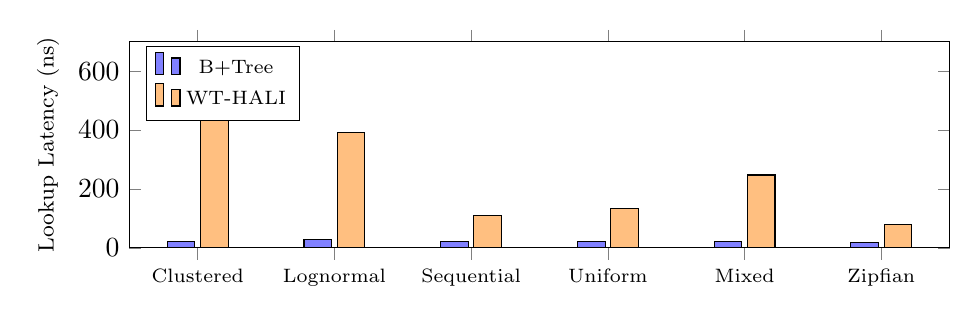
\begin{tikzpicture}
\begin{axis}[
    ybar,
    width=12cm, height=4.2cm,
    ylabel={\footnotesize Lookup Latency (ns)},
    symbolic x coords={Clustered, Lognormal, Sequential, Uniform, Mixed, Zipfian},
    xtick=data,
    xticklabel style={font=\scriptsize},
    ymin=0, ymax=700,
    legend style={at={(0.02,0.98)}, anchor=north west, font=\scriptsize},
    bar width=10pt,
    ylabel style={font=\footnotesize}
]
\addplot[fill=blue!50] coordinates {(Clustered,22.7) (Lognormal,28.3) (Sequential,20.2) (Uniform,22.2) (Mixed,21.1) (Zipfian,19.6)};
\addplot[fill=orange!50] coordinates {(Clustered,635.7) (Lognormal,391.1) (Sequential,110.9) (Uniform,132.9) (Mixed,247.4) (Zipfian,79.1)};
\legend{B+Tree, WT-HALI}
\end{axis}
\end{tikzpicture}
\end{center}

\vspace{0.1cm}

\begin{columns}
\column{0.48\textwidth}
\textbf{B+Tree:} Consistent 20-28ns (1.4$\times$ variance)\\
{\scriptsize Works equally well on any distribution}

\column{0.48\textwidth}
\textbf{WT-HALI:} 79-636ns (8$\times$ variance)\\
{\scriptsize Best on Sequential (111ns), worst on Clustered (636ns)}
\end{columns}

\vspace{0.1cm}

\begin{center}
\colorbox{yellow!20}{\parbox{11cm}{\centering \footnotesize 
\textbf{Implication:} WT-HALI excels on Sequential/Zipfian data (high R$^2$ $\rightarrow$ more PGM experts)\\
Struggles on Clustered data (irregular patterns $\rightarrow$ more ART fallback)
}}
\end{center}
\end{frame}

\begin{frame}{Trade-off Analysis: Memory vs Performance}
\textbf{Where does WT-HALI fit in the design space?}

\vspace{0.2cm}

\begin{center}
\scriptsize
\begin{tabular}{lcccl}
\toprule
\textbf{Index} & \textbf{Memory} & \textbf{Lookup} & \textbf{Insert} & \textbf{Best For} \\
& (B/key) & (ns) & (M/s) & \\
\midrule
B+Tree & 19.2 & \textcolor{green!70!black}{22.7} & \textcolor{green!70!black}{17.4} & General purpose \\
Hash & 41.8 & 183.3 & 13.9 & Point lookups, memory OK \\
ART & 20.0 & 393.9 & 13.7 & Variable-length keys \\
\midrule
RMI & \textcolor{green!70!black}{16.0} & 73.1 & \textcolor{red}{0.19} & Read-only, low memory \\
PGM & \textcolor{green!70!black}{16.0} & 155.7 & \textcolor{red}{0.18} & Read-only, low memory \\
\midrule
\rowcolor{yellow!20}
WT-HALI & 16.7 & 635.7 & 1.0 & \textbf{Memory-constrained + writes} \\
\bottomrule
\end{tabular}
\end{center}

\vspace{0.2cm}

\begin{columns}
\column{0.48\textwidth}
\begin{block}{WT-HALI Wins When:}
\scriptsize
\begin{itemize}
    \item Memory budget $<$ 17 B/key \textbf{AND}
    \item Need $>$ 180K writes/sec \textbf{AND}
    \item Can tolerate $>$ 500ns lookups
\end{itemize}
\end{block}

\column{0.48\textwidth}
\begin{block}{WT-HALI Loses When:}
\scriptsize
\begin{itemize}
    \item Need $<$ 100ns lookups (use B+Tree/RMI)
    \item Need $>$ 5M writes/sec (use B+Tree)
    \item Memory is not a constraint (use B+Tree)
\end{itemize}
\end{block}
\end{columns}

\vspace{0.1cm}

\begin{center}
\colorbox{blue!10}{\scriptsize \textbf{Key finding:} WT-HALI occupies a narrow but real niche: memory-constrained systems with moderate write requirements}
\end{center}
\end{frame}

% ============================================================
% SECTION 6: RECOMMENDATIONS
% ============================================================

\begin{frame}{When to Use What: Practical Guidelines}
\begin{center}
\scriptsize
\begin{tabular}{@{}p{3.5cm}p{2.2cm}p{5.5cm}@{}}
\toprule
\textbf{Scenario} & \textbf{Best Choice} & \textbf{Rationale} \\
\midrule
General purpose & \textbf{B+Tree} & Fastest, most predictable, battle-tested \\
Read-heavy, memory OK & \textbf{B+Tree} & 22ns lookups, 17M writes, range support \\
Read-heavy, low memory & \textbf{RMI/PGM} & 73-156ns lookups at 16 B/key \\
Write-heavy & \textbf{B+Tree/Hash} & 13-17M inserts/sec \\
\rowcolor{yellow!20}
Memory-constrained + writes & \textbf{WT-HALI} & 1M ins/sec at 16.7 B/key (5$\times$ better than PGM) \\
\rowcolor{yellow!20}
Sequential/time-series data & \textbf{WT-HALI} & High R$^2$ $\rightarrow$ fast PGM experts (79-111ns) \\
Range queries needed & \textbf{B+Tree} & Only option with efficient range support \\
Concurrent access & \textbf{B+Tree} & Fine-grained locking, well-understood \\
\bottomrule
\end{tabular}
\end{center}

\vspace{0.2cm}

\begin{columns}
\column{0.48\textwidth}
\begin{block}{WT-HALI Sweet Spot}
\scriptsize
\begin{itemize}
    \item Embedded/IoT devices (memory $<$ 20 B/key)
    \item Time-series databases (sequential timestamps)
    \item Append-mostly log systems (90\%+ writes)
    \item Edge computing with memory constraints
\end{itemize}
\end{block}

\column{0.48\textwidth}
\begin{block}{Avoid WT-HALI When}
\scriptsize
\begin{itemize}
    \item Need $<$50ns lookups (latency-critical)
    \item Need $>$10M writes/sec (high throughput)
    \item Random/clustered data distribution
    \item Production-critical systems (use proven B+Tree)
\end{itemize}
\end{block}
\end{columns}
\end{frame}

% ============================================================
% SECTION 7: LESSONS AND CONCLUSION
% ============================================================

\begin{frame}{Key Lessons for OS Design}
\begin{columns}
\column{0.55\textwidth}
\textbf{Three Core Findings:}

\vspace{0.15cm}

\begin{enumerate}
    \item \textbf{Write-through buffering works}
    \begin{itemize}
        \scriptsize
        \item 5$\times$ improvement over pure learned indexes
        \item Still 17$\times$ slower than B+Tree writes
        \item Amortized retrain cost is manageable (50-100ms)
    \end{itemize}
    
    \vspace{0.1cm}
    
    \item \textbf{Routing accuracy is critical}
    \begin{itemize}
        \scriptsize
        \item v1 probabilistic: 25-47\% $\rightarrow$ unusable in practice
        \item v2 deterministic: 100\% $\rightarrow$ predictable behavior
        \item Worth the +25\% lookup overhead for correctness
    \end{itemize}
    
    \vspace{0.1cm}
    
    \item \textbf{Memory savings often insufficient}
    \begin{itemize}
        \scriptsize
        \item Only 13\% savings (16.7 vs 19.2 B/key)
        \item 28$\times$ lookup slowdown is steep price
        \item Only worthwhile in truly constrained scenarios
    \end{itemize}
\end{enumerate}

\column{0.42\textwidth}
\textbf{OS Design Principles Validated:}

\vspace{0.15cm}

\begin{center}
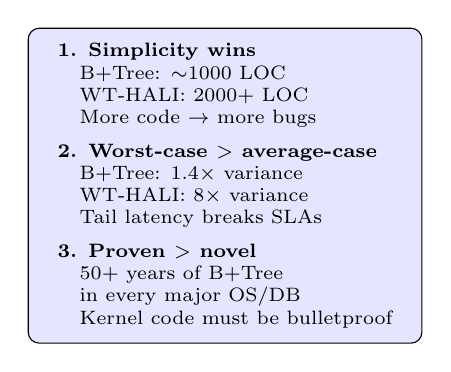
\begin{tikzpicture}
\node[draw, fill=blue!10, minimum width=5cm, minimum height=4cm, align=left, rounded corners, font=\scriptsize] {
    \textbf{1. Simplicity wins}\\
    \quad B+Tree: $\sim$1000 LOC\\
    \quad WT-HALI: 2000+ LOC\\
    \quad More code $\rightarrow$ more bugs\\[0.15cm]
    \textbf{2. Worst-case $>$ average-case}\\
    \quad B+Tree: 1.4$\times$ variance\\
    \quad WT-HALI: 8$\times$ variance\\
    \quad Tail latency breaks SLAs\\[0.15cm]
    \textbf{3. Proven $>$ novel}\\
    \quad 50+ years of B+Tree\\
    \quad in every major OS/DB\\
    \quad Kernel code must be bulletproof
};
\end{tikzpicture}
\end{center}
\end{columns}

\vspace{0.15cm}

\begin{center}
\colorbox{red!10}{\parbox{11cm}{\centering \footnotesize \textbf{Bottom line:} Hybrid approach improves on pure learned indexes, but cannot match traditional structures for general-purpose use}}
\end{center}
\end{frame}

\begin{frame}{Conclusion \& Future Work}
\begin{columns}
\column{0.48\textwidth}
\textbf{What We Built:}
\begin{itemize}
    \scriptsize
    \item Comprehensive benchmark: 6 indexes, 108 experiments
    \item Novel WT-HALI hybrid architecture
    \item Identified and fixed critical routing accuracy issue (v1$\rightarrow$v2)
    \item 100\% correctness validation on all experiments
    \item Fully reproducible Docker environment
\end{itemize}

\vspace{0.15cm}

\textbf{Key Contributions:}
\begin{itemize}
    \scriptsize
    \item Demonstrated 5$\times$ write improvement over pure learned
    \item Showed deterministic routing is essential for indexing
    \item Quantified memory vs performance trade-offs
    \item Identified specific use cases for hybrid indexes
\end{itemize}

\column{0.48\textwidth}
\textbf{Current Limitations:}
\begin{itemize}
    \scriptsize
    \item Single-threaded implementation only
    \item Point lookups only (no range query support)
    \item Tested on synthetic data (500K keys max)
    \item Still 17$\times$ slower writes than B+Tree
\end{itemize}

\vspace{0.15cm}

\textbf{Future Work:}
\begin{itemize}
    \scriptsize
    \item Scale testing: 1M-100M keys
    \item Real-world benchmarks: SOSD, YCSB
    \item Concurrent WT-HALI with fine-grained locks
    \item Range query support via sorted buffer
    \item Hardware acceleration (SIMD binary search)
\end{itemize}
\end{columns}

\vspace{0.2cm}

\begin{center}
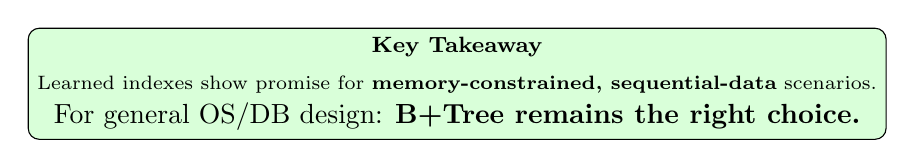
\begin{tikzpicture}
\node[draw, fill=green!15, minimum width=10cm, minimum height=1.3cm, align=center, rounded corners] {
    \footnotesize \textbf{Key Takeaway}\\[0.05cm]
    \scriptsize Learned indexes show promise for \textbf{memory-constrained, sequential-data} scenarios.\\
    For general OS/DB design: \textbf{B+Tree remains the right choice.}
};
\end{tikzpicture}
\end{center}

\vspace{0.1cm}

\begin{center}
\scriptsize
Dhruv Joshi (2022EE32079), Anushka Chaturvedi (2022EE31763)\\
ELL405: Operating Systems | IIT Delhi | Fall 2025\\
\textbf{Code:} \href{https://github.com/jdhruv1503/HALI}{\texttt{github.com/jdhruv1503/HALI}}
\end{center}
\end{frame}

\end{document}